\subsection{Risk Managment}
For this project, the ”Project Management Triangle” is lacking the cost dimension, while the time dimension is fixed (strict deadlines). As a result, any risks that appear, automatically lead to a reduction of the project scope if there is no spare time. Because of this, we will prioritize dealing with risks above regular tasks and prioritize essential tasks over nice-to-haves, but we do not intend on planning in a flat time margin as we have no way to negotiate for more time.

\subsection{Estimated Risks}
The numbers in the following picture describe the position of the risks on the following page from top to bottom.

\begin{figure}[H]
  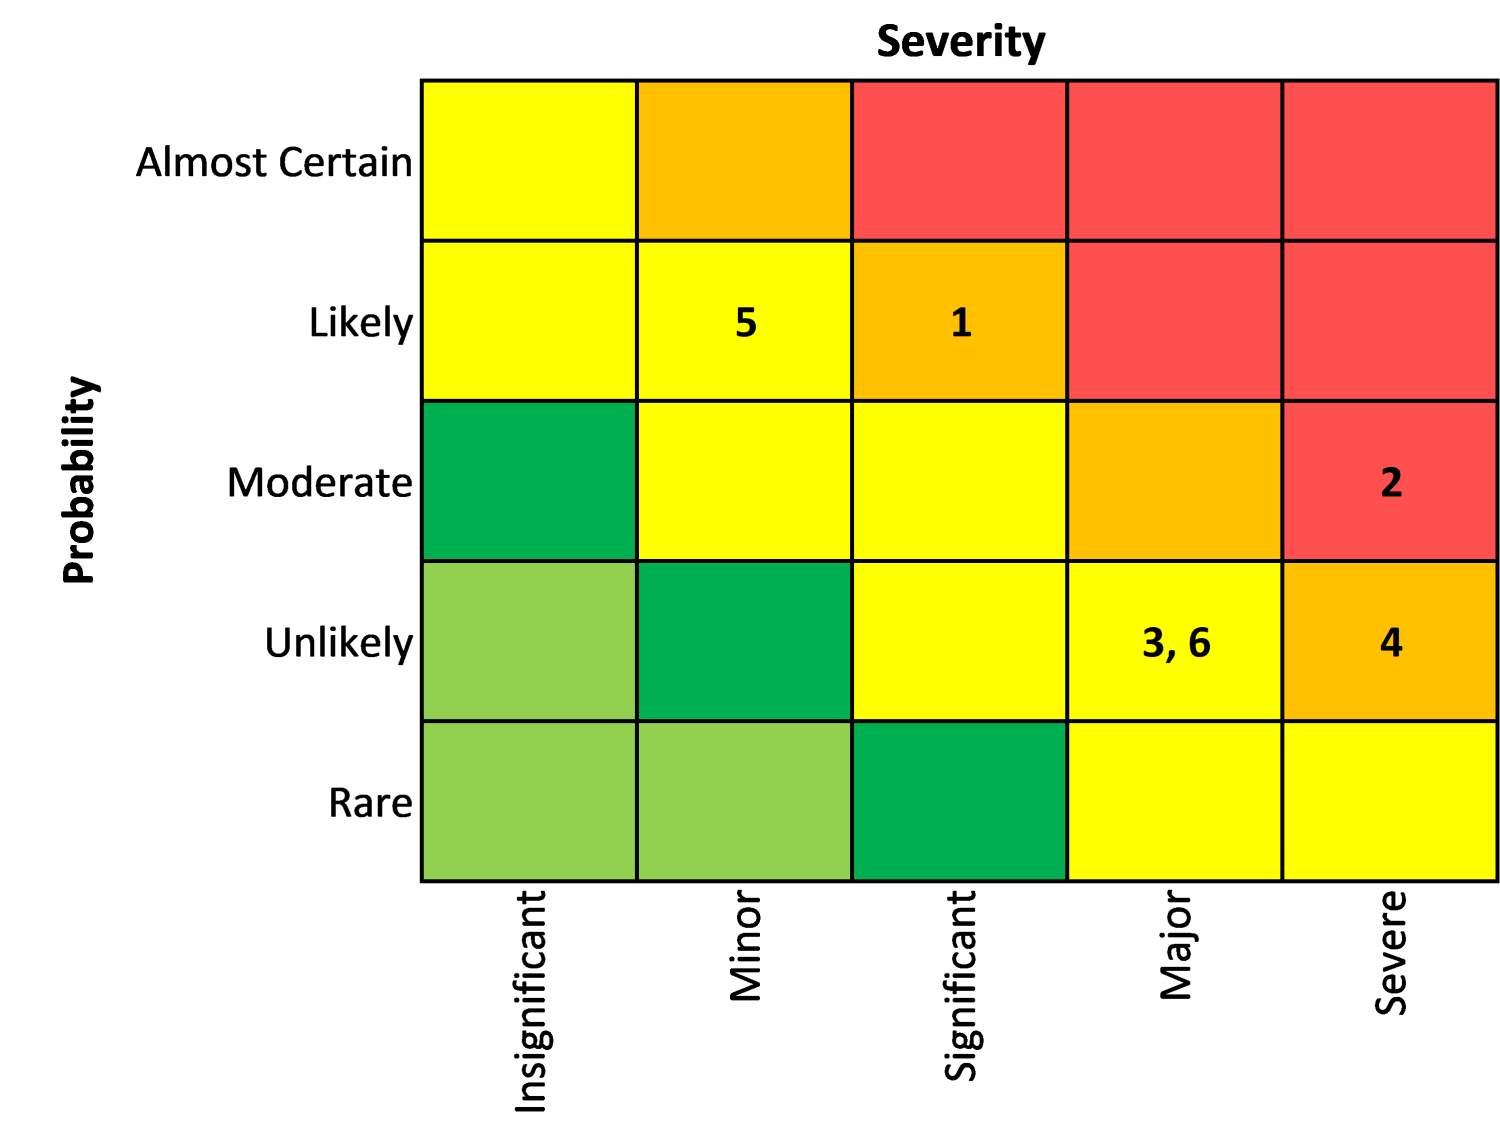
\includegraphics[width=\linewidth]{resources/risks-matrix.png}
  \caption{Risk matrix}
  \label{risk_matrix}
\end{figure}

\begin{table}
  \centering
  \begin{tabular}{|p{0.2\linewidth}p{0.7\linewidth}|}
    \hline
    \multicolumn{2}{|c|}{\textbf{Risk 1:}}                     \\
    Description     & Finding testing participants           \\
    Severity        & Medium                                 \\
    Probability     & High                                   \\
    Mitigations     & Already got confirmation from testers  \\
    New probability & Low                                    \\
    \hline                           
  \end{tabular}
  \caption{Testing participants risk}
\end{table}

\begin{table}
  \centering
  \begin{tabular}{|p{0.2\linewidth}p{0.7\linewidth}|}
    \hline
    \multicolumn{2}{|c|}{\textbf{Risk 2:}} \\
    Description     & Being able to create reversable programs with additional difficulties           \\
    Severity        & Very High                                 \\
    Probability     & Medium                                   \\
    Mitigations     & Assured the advisor is available for consultation  \\
    New probability & Low       \\
    \hline                            
  \end{tabular}
  \caption{Create programs risk}
\end{table}

\begin{table}
  \centering
  \begin{tabular}{|p{0.2\linewidth}p{0.7\linewidth}|}
    \hline
    \multicolumn{2}{|c|}{\textbf{Risk 3:}} \\
    Description            & Not enough time for the actual challenges because of too much programming etc.           \\
    Severity        & High                                 \\
    Probability     & Low                                   \\
    Mitigations     & Creating challenges in chronological order and in a iterating fashion  \\
    New probability & Very Low     \\
    \hline                              
  \end{tabular}
  \caption{Not enough time risk}
\end{table}

\newpage

\begin{table}
  \centering
  \begin{tabular}{|p{0.2\linewidth}p{0.7\linewidth}|}
    \hline
    \multicolumn{2}{|c|}{\textbf{Risk 4:}} \\
    Description     & Irreparable corruption of git server           \\
    Severity        & Very High                                 \\
    Probability     & Low                                   \\
    Mitigations     & Weekly off-site git server backups  \\
    New severity    & Low      \\
    \hline                             
  \end{tabular}
  \caption{Corruption of git risk}
\end{table}

\begin{table}
  \centering
  \begin{tabular}{|p{0.2\linewidth}p{0.7\linewidth}|}
    \hline
    \multicolumn{2}{|c|}{\textbf{Risk 5:}} \\
    Description     & Lost work due to unpushed work           \\
    Severity        & Low                                 \\
    Probability     & High                                   \\
    Mitigations     & Frequent reminders to push changes  \\
    New probability & Low   \\
    \hline                                
  \end{tabular}
  \caption{Unpushed work risk}
\end{table}

\begin{table}
  \centering
  \begin{tabular}{|p{0.2\linewidth}p{0.7\linewidth}|}
    \hline
    \multicolumn{2}{|c|}{\textbf{Risk 6:}} \\
    Description     & License problems with used software           \\
    Severity        & High                                 \\
    Probability     & Low                                   \\
    Mitigations     & Trying to use opensource or public software  \\
    New probability & Low       \\
    \hline                            
  \end{tabular}
  \caption{Licence problems risk}
\end{table}
